\documentclass{beamer}
\usepackage[utf8]{inputenc}

\usetheme{Madrid}
\usecolortheme{default}
\usepackage{amsmath,amssymb,amsfonts,amsthm}
\usepackage{txfonts}
\usepackage{tkz-euclide}
\usepackage{listings}
\usepackage{adjustbox}
\usepackage{array}
\usepackage{tabularx}
\usepackage{gvv}
\usepackage{lmodern}
\usepackage{circuitikz}
\usepackage{tikz}
\usepackage{graphicx}
\usepackage{multicol}

\setbeamertemplate{page number in head/foot}[totalframenumber]

\usepackage{tcolorbox}
\tcbuselibrary{minted,breakable,xparse,skins}



\definecolor{bg}{gray}{0.95}
\DeclareTCBListing{mintedbox}{O{}m!O{}}{%
	breakable=true,
	listing engine=minted,
	listing only,
	minted language=#2,
	minted style=default,
	minted options={%
		linenos,
		gobble=0,
		breaklines=true,
		breakafter=,,
		fontsize=\small,
		numbersep=8pt,
		#1},
	boxsep=0pt,
	left skip=0pt,
	right skip=0pt,
	left=25pt,
	right=0pt,
	top=3pt,
	bottom=3pt,
	arc=5pt,
	leftrule=0pt,
	rightrule=0pt,
	bottomrule=2pt,
	toprule=2pt,
	colback=bg,
	colframe=orange!70,
	enhanced,
	overlay={%
		\begin{tcbclipinterior}
			\fill[orange!20!white] (frame.south west) rectangle ([xshift=20pt]frame.north west);
	\end{tcbclipinterior}},
	#3,
}
\lstset{
	language=C,
	basicstyle=\ttfamily\small,
	keywordstyle=\color{blue},
	stringstyle=\color{orange},
	commentstyle=\color{green!60!black},
	numbers=left,
	numberstyle=\tiny\color{gray},
	breaklines=true,
	showstringspaces=false,
}
%------------------------------------------------------------
%This block of code defines the information to appear in the
%Title page
\title %optional
{2.10.78}
%\subtitle{A short story}

\author % (optional)
{Hema Havil - EE25BTECH11050}



\begin{document}
	
	\frame{\titlepage}
	\begin{frame}{Question}
		The point (4, 1) undergoes the following three transformations successively.\\
             (a) Reflection about the line $y = x$.\\
             (b) Translation through a distance 2 units along the positive direction of x-axis.\\
             (c) Rotation through an angle $\frac{\pi}{4}$ about the origin in the counter clockwise direction.\\
         Then the final position of the point is given by the coordinates.
         \begin{multicols}{2}
                (a) $\brak{\frac{1}{\sqrt{2}},\frac{7}{\sqrt{2}}}$
                (b) $\brak{-\sqrt{2},7\sqrt{2}}$
                (c) $\brak{\sqrt{2},7\sqrt{2}}$
                (d) $\brak{-\frac{1}{\sqrt{2}},\frac{7}{\sqrt{2}}}$
         \end{multicols}
	\end{frame}

	
\begin{frame}{Theoretical Solution}
	Let the given point be P=(4,1) and vector be $\vec{P}=\myvec{4\\1}$,\\
             (a) Reflection matrix for $y=x$ is,
             \begin{align}
                 \vec{M}=\myvec{0\;1\\1\;0}
             \end{align}
             then the reflection of P about $y=x$ is,
             \begin{align}
                 \vec{P_1}=\vec{M}\vec{P}
             \end{align}
             \begin{align}
                 \vec{P_1}=\myvec{0\;1\\1\;0}\myvec{4\\1}
             \end{align}
             \begin{align}
                 \vec{P_1}=\myvec{1\\4}
             \end{align}
             
\end{frame}
\begin{frame}{Theoretical Solution}
(b) Translate point $P_1=(1,4)$, 2 units along the positive direction of x axis,
             \begin{align}
                 \vec{P_2} = \vec{P_1} + \vec{X}
             \end{align}
             where X=(2,0)
             \begin{align}
                 \vec{P_2} = \myvec{1\\4}+\myvec{2\\0}
             \end{align}
             \begin{align}
                 \vec{P_2} = \myvec{3\\4}
             \end{align}
             (c) Rotation matrix is given as,
             \begin{align}
                 \vec{R}=\myvec{cos\theta\;-sin\theta\\sin\theta\;\;\;\;\;cos\theta}
             \end{align}
             
	\end{frame}
    \begin{frame}{Theoretical Solution}
             Rotation of $P_2$ by an angle $\frac{\pi}{4}$ about the origin in the counter clockwise direction, substitute $\frac{\pi}{4}$ in R
             \begin{align}
                 \vec{P_3}=\vec{R}\vec{P_2}
             \end{align}
             \begin{align}
                 \vec{P_3}=\myvec{\frac{1}{\sqrt{2}}\;-\frac{1}{\sqrt{2}}\\\frac{1}{\sqrt{2}}\;\;\;\;\frac{1}{\sqrt{2}}}\myvec{3\\4}
             \end{align}
             \begin{align}
                 \vec{P_3}=\myvec{-\frac{1}{\sqrt{2}}\\\frac{7}{\sqrt{2}}}
             \end{align}
             Therefore the final position of the point is $P_3=(-\frac{1}{\sqrt{2}},\frac{7}{\sqrt{2}})$, option (d) is correct
    \end{frame}
	\begin{frame}[fragile]
	\frametitle{C Code- Computing the unit vector}
	
	\begin{lstlisting}
/// File: transform.c
#include <stdio.h>

void matvec2x2(double mat[2][2], double vec[2], double result[2]) {
    for (int i = 0; i < 2; i++) {
        result[i] = 0;
        for (int j = 0; j < 2; j++) {
            result[i] += mat[i][j] * vec[j];
        }
    }
}




	\end{lstlisting}
\end{frame}
\begin{frame}[fragile]
\frametitle{C Code - Computing the unit vector}
\begin{lstlisting}
    void matvec3x3(double mat[3][3], double vec[3], double result[3]) {
    for (int i = 0; i < 3; i++) {
        result[i] = 0;
        for (int j = 0; j < 3; j++) {
            result[i] += mat[i][j] * vec[j];
        }
    }
}
\end{lstlisting}
\end{frame}

\begin{frame}[fragile]
	\frametitle{Python Code using shared output}
    \scriptsize
	\begin{lstlisting}
		import ctypes
import numpy as np
import matplotlib.pyplot as plt

# Load C shared library
lib = ctypes.CDLL('./libtransform.so')

# Set argument and return types
lib.matvec2x2.argtypes = [np.ctypeslib.ndpointer(dtype=np.float64, shape=(2,2)),
                          np.ctypeslib.ndpointer(dtype=np.float64, shape=(2,)),
                          np.ctypeslib.ndpointer(dtype=np.float64, shape=(2,))]
	\end{lstlisting}
\end{frame}
\begin{frame}[fragile]
	\frametitle{Python Code using shared output}
	\begin{lstlisting}	
    lib.matvec3x3.argtypes = [np.ctypeslib.ndpointer(dtype=np.float64, shape=(3,3)),
                          np.ctypeslib.ndpointer(dtype=np.float64, shape=(3,)),
                          np.ctypeslib.ndpointer(dtype=np.float64, shape=(3,))]
     # Initial point
P = np.array([4.0, 1.0])

# Step 1: Reflection over y = x → swap x and y
reflect_mat = np.array([[0.0, 1.0],
                        [1.0, 0.0]])
P1 = np.zeros(2)
lib.matvec2x2(reflect_mat, P, P1)
	\end{lstlisting}
\end{frame}
\begin{frame}[fragile]
	\frametitle{Python Code using shared output}
	\begin{lstlisting}
    # Step 2: Translation +2 in x-direction using 3x3 matrix
P1_h = np.array([P1[0], P1[1], 1.0])
translate_mat = np.array([[1.0, 0.0, 2.0],
                          [0.0, 1.0, 0.0],
                          [0.0, 0.0, 1.0]])
P2_h = np.zeros(3)
lib.matvec3x3(translate_mat, P1_h, P2_h)
P2 = P2_h[:2]

# Step 3: Rotation by pi/4 (45° counterclockwise)
theta = np.pi / 4
cos_t = np.cos(theta)
sin_t = np.sin(theta)
rotation_mat = np.array([[cos_t, -sin_t],
                         [sin_t, cos_t]])
P3 = np.zeros(2)
lib.matvec2x2(rotation_mat, P2, P3)
	\end{lstlisting}
\end{frame}
\begin{frame}[fragile]
        \frametitle{Python Code using shared output}
        \begin{lstlisting}
        # Plotting the transformation steps
points = np.array([P, P1, P2, P3])
labels = ['Original (4,1)', 'After Reflection', 'After Translation', 'After Rotation (Final)']
colors = ['blue', 'orange', 'green', 'red']
plt.figure(figsize=(8, 8))
            
for i, point in enumerate(points):
    plt.plot(point[0], point[1], 'o', label=labels[i], color=colors[i])
    plt.text(point[0]+0.1, point[1]+0.1, f'{labels[i]}')
        \end{lstlisting}
\end{frame}
\begin{frame}[fragile]
   \frametitle{Frame Title}
    \begin{lstlisting}
        plt.plot(points[:,0], points[:,1], '--k', alpha=0.5)
plt.grid(True)
plt.axhline(0, color='black', lw=1)
plt.axvline(0, color='black', lw=1)
plt.legend()
plt.title("Transformation of Point (4,1)")
plt.xlabel("X")
plt.ylabel("Y")
plt.axis('equal')
plt.show()

# Final result
print(f"Final coordinates after all transformations: ({P3[0]}, {P3[1]})")
    \end{lstlisting}
\end{frame}
\begin{frame}{Plot by python using shared output from c}
	\begin{center}
	\begin{figure}[H]
		\centering
		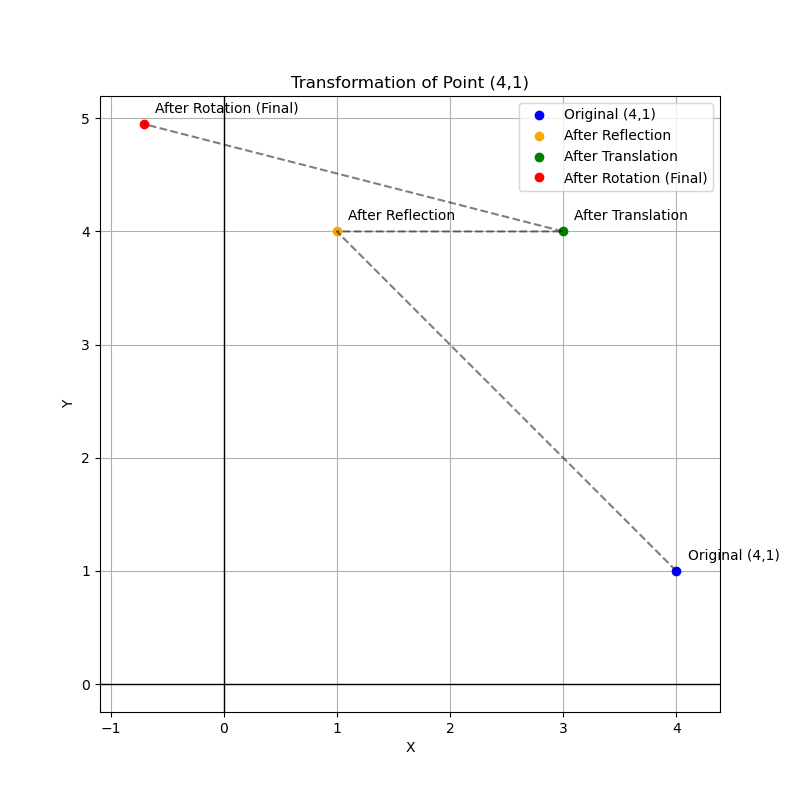
\includegraphics[width = 0.5\columnwidth]{figs/fig1.png}
		\caption{Plot for the transformations of P}
		\label{fig1}
	\end{figure}
	\end{center}
\end{frame}
\begin{frame}[fragile]
   \frametitle{Python code for the plot}
    \begin{lstlisting}
import numpy as np
import matplotlib.pyplot as plt

# Step 0: Initial point
P = np.array([4.0, 1.0])
points = [P]
labels = ["Original (4,1)"]

# Step 1: Reflection about the line y = x
# Matrix: [[0, 1], [1, 0]]
reflect_matrix = np.array([[0, 1],
                           [1, 0]])
P1 = reflect_matrix @ P
points.append(P1)
labels.append("After Reflection")


 \end{lstlisting}
\end{frame}
 \begin{frame}[fragile]
       \frametitle{Python code for plot}
       \begin{lstlisting}
      # Step 2: Translation by 2 units along +x-axis
# Use homogeneous coordinates: convert P1 to 3D vector
P1_h = np.array([P1[0], P1[1], 1.0])
translate_matrix = np.array([[1, 0, 2],
                             [0, 1, 0],
                             [0, 0, 1]])
P2_h = translate_matrix @ P1_h
P2 = P2_h[:2]
points.append(P2)
labels.append("After Translation")

# Step 3: Rotation by π/4 counter-clockwise
theta = np.pi / 4
cos_t = np.cos(theta)
sin_t = np.sin(theta)
rotate_matrix = np.array([[cos_t, -sin_t],
                          [sin_t, cos_t]])


    \end{lstlisting}
 \end{frame}
 \begin{frame}[fragile]
   \frametitle{Python code for plot}
     \begin{lstlisting}
         P3 = rotate_matrix @ P2
points.append(P3)
labels.append("After Rotation ")

# Convert all points to a NumPy array
points = np.array(points)

# Plotting
colors = ['blue', 'orange', 'green', 'red']
plt.figure(figsize=(8, 8))
for i, point in enumerate(points):
    plt.plot(point[0], point[1], 'o', color=colors[i], label=labels[i])
    plt.text(point[0] + 0.2, point[1] + 0.2, f"{labels[i]}\n({point[0]:.2f}, {point[1]:.2f})")
# Draw arrows between steps
   for i in range(len(points) - 1):
     \end{lstlisting}
 \end{frame}
 \begin{frame}[fragile]
    \frametitle{Python code for the plot}
     \begin{lstlisting} 
    plt.arrow(points[i][0], points[i][1],
              points[i+1][0] - points[i][0],
              points[i+1][1] - points[i][1],
              head_width=0.2, length_includes_head=True,
              fc='gray', ec='gray', linestyle='dashed')

plt.axhline(0, color='black', linewidth=1)
plt.axvline(0, color='black', linewidth=1)
plt.grid(True)
plt.legend()
plt.axis('equal')
plt.title("Transformations of Point (4, 1)")
plt.xlabel("X-axis")
plt.ylabel("Y-axis")
plt.show()

# Final output
print(f"Final coordinates: ({P3[0]:.4f}, {P3[1]:.4f})")
     \end{lstlisting}
 \end{frame}
 \begin{figure}[h]
     \centering
     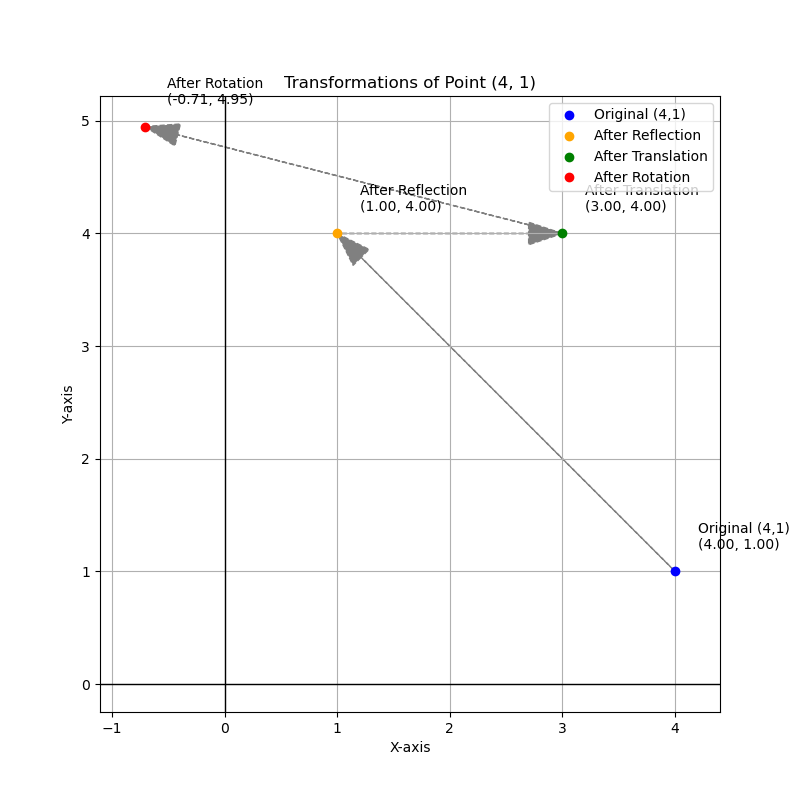
\includegraphics[width=0.7\linewidth]{figs/fig2.png}
     \caption{Plot for the transformations of P}
     \label{fig2}
 \end{figure}
\end{document}

